%% The first command in your LaTeX source must be the \documentclass command.
%%
%% Options:
%% twocolumn : Two column layout.
%% hf: enable header and footer.
\documentclass[
% twocolumn,
% hf,
]{ceurart}

%%
%% One can fix some overfulls
\sloppy

\usepackage{my-main-style}

%%
%% Minted listings support 
%% Need pygment <http://pygments.org/> <http://pypi.python.org/pypi/Pygments>
\usepackage{listings}
%% auto break lines
\lstset{breaklines=true}

%%
%% end of the preamble, start of the body of the document source.
\begin{document}

%%
%% Rights management information.
%% CC-BY is default license.
\copyrightyear{2025}
\copyrightclause{Copyright for this paper by its authors.
  Use permitted under Creative Commons License Attribution 4.0
  International (CC BY 4.0).}

%%
%% This command is for the conference information
\conference{HyperAgents'25: 2nd Workshop on Hypermedia Multi-Agent Systems,
  October 25-30, 2025, Bologna, Italy}

%%
%% The "title" command
\title{The Gap Between BDI Agents and Semantic Hypermedia and What We Can Do About It}

% \tnotemark[1]
% \tnotetext[1]{You can use this document as the template for preparing your
%   publication. We recommend using the latest version of the ceurart style.}

%%
%% The "author" command and its associated commands are used to define
%% the authors and their affiliations.
\author[1]{Samuele Burattini}[%
orcid=0009-0009-4853-7783,
email=samuele.burattini@unibo.it,
]
\cormark[1]
\fnmark[1]

\author[1]{Martina Baiardi}[%
orcid=0009-0001-0799-9166,
email=m.baiardi@unibo.it,
]
\fnmark[1]

\author[1]{Giovanni Ciatto}[%
orcid=0000-0002-1841-8996,
email=giovanni.ciatto@unibo.it,
]


\author[1]{Danilo Pianini}[%
orcid=0000-0002-8392-5409,
email=danilo.pianini@unibo.it,
]



\address[1]{\disi, \unibo}


%% Footnotes
\cortext[1]{Corresponding author.}
\fntext[1]{These authors contributed equally.}

%%
%% The abstract is a short summary of the work to be presented in the
%% article.
\begin{abstract}
  Traditional BDI agents, 
  rooted in logic programming, 
  remain poorly integrated with the hypermedia nature of open Web environments
  which typically rely on Semantic Web technologies such as RDF and OWL.
  This paper examines the gap between these paradigms and surveys existing integration efforts on a conceptual and technical level.
  Our proposal for a deeper integration relies on a generalized BDI engine to enable the development of BDI agents that can directly reason and operate on semantic hypermedia resources.
  We reflect on the potential benefits and challenges of this approach and show preliminary results of a proof-of-concept implementation.
\end{abstract}

%%
%% Keywords. The author(s) should pick words that accurately describe
%% the work being presented. Separate the keywords with commas.
\begin{keywords}
  BDI  \sep 
  Hypermedia \sep 
  Agent-Oriented Programming
\end{keywords}

%%
%% This command processes the author and affiliation and title
%% information and builds the first part of the formatted document.
\maketitle

%==========================================================
\section{Introduction}
%==========================================================

Integrating intelligent agents with the Web is a long-standing goal
in both the \ac{MAS}~\cite{DBLP:conf/edoc/ShafiqDF06}
and Semantic Web~\cite{lassila2001semantic} communities, but,
despite such common interest, 
the famous question ``Where are all the intelligent agents?'' remains unanswered to this day~\cite{hendlerb2007expert}.

In the last decade, developments in the engineering of Web services including
the more pervasive use of hypermedia and the \ac{REST} architectural style~\cite{DBLP:journals/toit/FieldingT02},
and the growing adoption of Web interoperability standards even outside the traditional Web domain
-- such as the \ac{WoT}~\cite{wotarch} --
has renewed the interest in the integration of \ac{MAS} and the Web.
%
In this context, 
the proposal of \ac{hMAS}~\cite{DBLP:conf/atal/CiorteaMGBRZ19} suggested a new perspective
envisioning the Web itself as an open environment
which agents can roam by consuming and manipulating hypermedia resources.
%
As an outcome of the resurgence of Web \ac{MAS},
the \ac{W3C} Autonomous Agents on the Web community group\footnote{\url{https://www.w3.org/community/webagents/}}
has been founded to connect researchers and practitioners working in the area. 

Even more recently, the advent of \ac{LLM} and the \emph{Agentic AI} movement~\cite{acharya2025access} 
have taken by storm the development of intelligent agents that interact with the Web by invoking Web APIs~\missingref{} and interpreting natural language content~\missingref{}.
%
Despite these approaches showing promising results,
they do not yet replace the controllability of traditional agent-programming paradigms~\missingref{},
nor they make obsolete the need for structured knowledge representation and reasoning~\cite{pan2024tkde} provided by Semantic Web technologies such as the \ac{RDF}~\cite{RDF_Concepts_W3C:14} and \ac{OWL}~\cite{OWL_Syntax_W3C:12}.
%
Agents developed with cognitive architectures such as the \ac{BDI} model
capable of leveraging structured knowledge within the Semantic Web 
hence remain a valid approach for the development of intelligent systems on the Web.

We argue that the integration of \ac{BDI} agents with the Web
is hindered by a conceptual and technological gap, 
which limits developers in creating agents that can effectively reason and operate on semantic hypermedia resources.
Namely:
\begin{enumerate}[label={(G\arabic*)}]
  \item \ac{BDI} agents have typically been tied to logic programming
  %-- e.g., with the popular \agentspeak{} semantic~\cite{DBLP:conf/maamaw/Rao96} --
  whereas the Semantic Web is grounded on \ac{DL}. The different technological choices used to concretely implement them add cognitive load to developers working on the integration of the two worlds (e.g., converting \ac{OWL} and \ac{RDF} triples in Prolog-like formulas);
  \label{gap:logic}
  \item \ac{BDI} agents are typically implemented with the \ac{PRS} architecture~\cite{georgeff1986pieee} which relies on pre-defined plans and hence provides limited support for the exploitation of new action possibilities discovered in an open hypermedia environment.
  \label{gap:open-world}
\end{enumerate}

In this paper, we reflect on these gaps and their technical implications on the overall development experience of creating \ac{BDI} agents that interact with Web resources and how this can be mitigated through the design of agent-oriented programming languages and frameworks. 

We start by providing a brief overview of the \ac{BDI} model, the hypermedia nature of the (Semantic) Web and the fundamental principles of \ac{hMAS} in \Cref{sec:background}.
%
We then analyze the gap between \ac{BDI} agents and hypermedia in \Cref{sec:gap-analysis}.
%
Then,
in \Cref{sec:integrating-bdi-hypermedia},
we identify ideal integration requirements and let those guide our analysis of existing approaches that have attempted to bridge the gap between \ac{BDI} agents and hypermedia in the past to understand limitations and potential room for improvement.
%
Finally, in \Cref{sec:generalized-bdi-engine} we present our research direction
aiming to tighten the integration of \ac{BDI} agents and hypermedia
and reduce the abstraction gap for developers 
by introducing a generalized \ac{BDI} engine
that can directly leverage Semantic Web technologies for belief representation and reasoning processes.
%
We show preliminary results of a proof-of-concept implementation
and discuss open challenges and opportunities of this approach.

%==========================================================
\section{Background}
\label{sec:background}
%==========================================================

\subsection{BDI Agents}

The \ac{BDI} model~\cite{DBLP:conf/atal/GeorgeffPPTW98}
is a well-established cognitive architecture for the development of intelligent agents.
%
% It is based on the idea of representing an agent's mental state in terms of three key components:
% \begin{inlinelist}
%   \item \emph{beliefs} are what the agent thinks to be true,
%   \item \emph{desires} are the potential goals or objectives an agent may pursue,
%   \item \emph{intentions} are the agent's commitments to achieve specific desires.
% \end{inlinelist}
\ac{BDI} agents follow a continuous cycle of
\begin{inlinelist}
  \item \emph{perception} of external stimuli and gather new \emph{beliefs},
  \item \emph{deliberation} to update beliefs, goals and choose \emph{intentions} to pursue selecting \emph{plan} to achieve goals,
  and
  \item \emph{action} advancing one intention by executing a step of the associated plan.
\end{inlinelist}
Practically, most \ac{BDI} agents implementations follow the \ac{PRS} architecture~\cite{georgeff1986pieee},
which is based on the ability for agents to select plans from a predefined set
and execute them to achieve their goals.

To declaratively define the agent's behavior the \ac{AOP} community has developed several \ac{BDI} programming languages and frameworks~\cite{DBLP:conf/woa/MascardiDA05}.
%
Arguably, the most popular language is \agentspeak{}~\cite{DBLP:conf/maamaw/Rao96} which 
uses a logic-based formal syntax and semantics for representing beliefs, goals and actions using logic predicates.
%This allows to exploit logic unification to query the agent's \emph{belief base} and match plans to achieve goals.
%The \agentspeak{} abstract language has been implemented in the \jason{}~\cite{bordini2007programming} agent programming platform, providing an interpreter and a Java-based runtime environment for developing \ac{BDI} \ac{MAS}.

% The logic-based nature of \agentspeak{} has characterized the development of \ac{BDI} agents due to its expressiveness and flexibility in supporting the basic mechanisms of the \ac{BDI} reasoning cycle.
%
Despite variations of \ac{BDI} programming languages and frameworks have been implemented without such a strong reliance on logic-based mechanisms (e.g., \cite{map2005sp,kampik2019emas}), in the following when we refer to \ac{BDI} agents we will implicitly refer to \agentspeak{}-like agents.

\subsection{The Web, Semantics and Hypermedia}

The World Wide Web was proposed by Tim Berners-Lee as a global, open information space
based on the ability to link resources through hypermedia documents~\cite{DBLP:journals/cn/Berners-LeeCG92}.
%
The Web is built with the \ac{REST} architectural style~\cite{DBLP:journals/toit/FieldingT02}
which supports independently evolving components through a set of principles.
%
% The \ac{REST} architectural style~\cite{DBLP:journals/toit/FieldingT02}
% adopted by the Web allows to have independently evolving components
% that can interact through a uniform interface thanks to:
% \begin{inlinelist}
%   \item \acp{URI} to identify resources,
%   \item the exchange of representations of resources using shared data formats (e.g., JSON, XML),
%   \item self-descriptive messages following the semantics of the HTTP protocol, and
%   \item the use of \ac{HATEOAS} guiding clients in their next possible actions.
% \end{inlinelist}

The Semantic Web~\cite{BernersLee2001} complements the \emph{self-descriptive} principle of \ac{REST} 
by encoding semantics in the representation through the general model of \ac{RDF}~\cite{RDF_Concepts_W3C:14}
based on machine-readable \emph{triples}
that state facts using a common vocabulary defined within ontologies, encoded in {OWL}~\cite{OWL_Syntax_W3C:12}.
%
%Ontologies can be used to encode structured knowledge about a domain of interest, creating consensus on the meaning of concepts and relationships between them, hence improving interoperability between different systems on the open Web.

Another fundamental principle is \ac{HATEOAS} which defines hypermedia as ``the simultaneous presentation of information and controls such that the information becomes the affordance through which the user obtains choices and selects actions''~\cite{DBLP:journals/toit/FieldingT02}.
% %
% Affordances
% -- i.e., action possibilities --
% are central to the inner workings of the Web,
% allowing clients to discover new resources and actions by consuming hypermedia.
% This mechanism drives the state transitions of the distributed client-server system
% ensuring scalability and independence of individual components.
In this way, the Web can be seen as an open environment
where clients discover new resources and action possibilities by consuming hypermedia.

When such hypermedia is annotated with explicit semantics it should be possible for clients to better understand the meaning of the affordances, avoiding the need for hard-coded knowledge.
%
%This is the mechanism adopted for instance in the \ac{WoT}~\cite{wotarch} where \emph{\ac{TD}} are used as semantic hypermedia representations of \ac{IoT} devices,
%declaring the possible interaction affordances exposed by the devices (e.g., reading a sensor value, turning on a light, etc.).


\subsection{Hypermedia Multi-Agent Systems}

\sbnote{Very briefly introduce the research context of hMAS}

%==========================================================
\section{Gap Analysis}
\label{sec:gap-analysis}
%==========================================================

From the brief background presented in \Cref{sec:background}, 
it should be evident that
despite both \ac{BDI} agents and the Semantic Web being rooted in logic-based knowledge representation,
there are significant differences between the two worlds.
%Specifically, Prolog-like logic typically used to practically implement \ac{BDI} agents and \ac{DL} used in the Semantic Web are different subsets of \ac{FOL} with consequently different expressiveness and semantics
Specifically, description logic excel in representing relationships between concepts, while \ac{BDI} agents use logic programming to store facts about the external environment as belief and declaratively express goals.
The different technologies used in the two different paradigms makes them difficult to integrate \ref{gap:logic}.
%
Furthermore, \ac{BDI} agents are typically designed with a closed-world perspective whereas the Semantic Web is an open information space \ref{gap:open-world}.
%
When it comes to practical applications this creates an abstraction and technological gap
which can be difficult to bridge for developers.
%
In the following, we describe in more detail such differences.

\paragraph{Syntactical Differences}

On a syntactical level, \ac{BDI} agents represent beliefs and goals using logic formulas
%which are either atomic \emph{terms} (e.g., \textsf{alice}) or a \emph{structure} composed of a \emph{functor} followed by an arbitrary number of \emph{arguments} within parentheses
(e.g. \textsf{person(alice)}).
%
Differently, in the Semantic Web, knowledge is represented in the form of \emph{triples} which connect a \emph{subject} to an \emph{object} through a \emph{predicate} (e.g. \textsf{:alice rdf:type foaf:Person}).
%
Although \ac{RDF} triples can be mapped to logic formulas, from a practical point of view, the degrees of freedom of this mapping can lead to a variety of seemingly ``semantically equivalent'' representations (e.g., \textsf{type(alice, person)} and \textsf{triple(alice, type, person)} are reasonable mappings of the \ac{RDF} triple above).
%
Developers wishing to integrate \ac{BDI} agents with the Semantic Web hence face the challenges of choosing a suitable -- and more importantly consistent -- mapping which we believe adds a significant cognitive load during the development process.

\paragraph{Semantics and Reasoning}
\ac{RDF} and \ac{OWL} provides a set of \emph{axioms} that define the meaning of the triples and how they can be inferred (e.g., \textsf{rdf:type} is a predicate that specify an \emph{instance of} relationship between the subject and a class).
%
When using \emph{ontologies} to represent standardized knowledge (e.g., \textsf{foaf}\footnote{\url{http://xmlns.com/foaf/spec/}} in the example above), 
the semantics of the triples is further defined by the ontology itself,
which can include additional axioms, constraints, and relationships between concepts.
%
This means that, in order to properly reason about the knowledge represented in \ac{RDF} and \ac{OWL},
developers may need to translate the whole \ac{RDF}, \ac{OWL} and ontology semantics into their own belief base, adding a significant overhead and a potential source of inconsistencies. 
Although \ac{OWL} ontologies can be converted into logic formulas through an automatic process~\cite{samuel2008tplp}
it can be cumbersome for \ac{BDI} developers to exploit them when writing the agent program
and similarly hard for Semantic Web experts to understand how to properly interact with the translated knowledge base.

\paragraph{Querying and Inference}

The logic representation used in \ac{BDI} agents supports querying the belief base using logic unification.
%
This basic mechanism allows to easily verify conditions based on the current beliefs, retrieve information and also perform inference using dedicated rules developers can encode to represent the problem domain.
%
Unification relies on finding a substitution for the variables in a logic formula that makes it true with the facts within a logic theory. When multiple substitutions are possible, the unification process usually returns the first available one, as it is typically implemented as a depth-first search algorithm with backtracking.
%
In contrast, the Semantic Web relies on \acs{SPARQL}~\cite{sparqlprotocol} to query \ac{RDF} data.
\acs{SPARQL} allows matching graph patterns and retrieve all the values of variables in the pattern from the matched triples, 
providing an intuitive way to query the knowledge base.
%
As for inference, given the expressiveness limitations of \ac{OWL}, the \ac{SWRL} can be used to extend it and define Prolog-like inference rules.
%
An important difference is that while logic unification automatically performs inference, \acs{SPARQL} searches only on the set of triples currently in a knowledge base. If inference is required, the developer must explicitly \emph{materialize} the triples inferred by a reasoner before querying.


\paragraph{Open vs. Close Environments}
\ac{BDI} agents are equipped with a predefined set of plans, composed of sequences of actions that the agent knows how to execute.
%
Additionally, \ac{BDI} agents usually run in a closed environment,
which is designed by the developer to provide perceptions to the agents and 
support the execution of the actions used in the plans~\cite{weyns2007aamas}. 
%
The development process of \ac{BDI} agents is hence based on the fact that a developer anticipates 
the relevant possible settings an agent may encounter and provides plans to handle them.
%
This makes it difficult for agents to adapt to unexpected settings or to flexibly incorporate new actions that become available while exploring the environment.
%
Relating this to the open hypermedia nature of the Web, makes the effective integration of \ac{BDI} agents challenging.
%
Following the \ac{HATEOAS} principle, agents may discover new affordances
-- i.e., action possibilities --
while navigating through the hypermedia environment.
%
The inability to exploit such new affordances may limit the agent in its ability to adapt to the environment and effectively interact with it.


%==========================================================
\section{Integrating \acs{BDI} Agents and Semantic Hypermedia}
\label{sec:integrating-bdi-hypermedia}
%==========================================================


Guided by the analysis of the gap between \ac{BDI} agents and semantic representation of hypermedia resources,
we identify a set of requirements that we believe may level such gap for practical development of \ac{BDI} agents in Web environments.
We hence propose that a \ac{BDI} agent programming framework for \ac{hMAS} should support the following features:
\begin{enumerate}[label={(R\arabic*)}]
  \item direct manipulation of \ac{RDF} and \ac{OWL} triples in the agent's belief base;
  \label{req:first}
  \item ontological reasoning and inference for plan selection;
  \label{req:second}
  \item support for querying the belief base using \ac{SPARQL} instead of logic unification;
  \label{req:third}
  \item ability to exploit affordances discovered in the environment to dynamically adapt the agent's plans.
  \label{req:fourth}
\end{enumerate}
\subsection{Existing Approaches}
\label{subsec:existing-approaches}
\sbnote{Related works, JASDL (Jason+Ontological reasoning), Yggdrasil framework, Hypermedea (Saint-Etienne Cartago Artifacts for Hypermedia), others.... }

\paragraph{Semantic extensions of AgentSpeak}
In \cite{DBLP:conf/dalt/MoreiraVBH05} authors propose an AgentSpeak extension named AgentSpeak-DL, 
where the belief base concepts are extended with the addition of \ac{DL}.
%
With the \ac{DL} extension, 
AgentSpeak-DL supports the definition of more structured objects and relationships between them, 
rather than only logic terms.
%
The semantics of AgentSpeak-DL demonstrates that agent-oriented programming can be extended for the development of Semantic Web applications, 
easing their adaptation to applications such as Grid Computing and Ubiquitous Computing.
%
In line with the requirements in~\Cref{subsec:integration-requirements}, 
authors highlight that changing the belief representation affects three operations of the whole AgentSpeak lifecycle, namely: the plan research, the query on the Belief Base, and the Belief Update.

\paragraph{Integration of DL in BDI engines}
The semantic extension AgentSpeak-DL proposed in~\cite{DBLP:conf/dalt/MoreiraVBH05}, 
is set to ground in JASDL~\cite{DBLP:conf/dalt/KlapiscakB08}.
%
In this work, 
authors provide an extension of \jason{} \ac{BDI} engine, 
where core elements are customised to welcome \ac{DL} semantics.
%
The latter is represented as a ``semantically-enriched'' literal,
represented inside the agent's belief base using FOL notation.
%
This choice allow to use \jason{}'s standard belief base selection mechanisms, 
and adds on top of them a reasoning engine that query the ontology instance.
%
The choice to represent \ac{DL} in this way in the engine has the advantage that make use of fullfledged \jason{} engine features.
%
However, 
this hindered the direct integration of the operational semantics described in~\cite{DBLP:conf/dalt/KlapiscakB08} 
and required technological workarounds to integrate it.
\mbnote{I know that ``workaround'' is not a good way to say this, I will improve the form}
%

\sbnote{for R4 we can mention the work from Danai on Signifiers, \cite{MeneguzziS15} for basic notions of planning and \cite{schmid2024kgswc} which is not BDI but has some interesting ideas on affordances and planning in hypermedia}

%==========================================================
\section{Levelling the Gap with a Generalised BDI Engine}
\label{sec:generalized-bdi-engine}
%==========================================================

In this section,
we propose a new approach to bridge the identified gaps between \ac{BDI} agents and semantic hypermedia resources,
guided by the requirements identified in \Cref{sec:integrating-bdi-hypermedia}.
%
The approach addresses mainly the first gap \ref{gap:logic}, 
and we believe it represents a first step towards addressing the second gap \ref{gap:open-world} as future work,
particularly by enabling more expressive \ac{BDI} frameworks.
%
The core idea is to introduce a generalised \ac{BDI} engine that encapsulates agents reasoning cycle, 
while decoupling the representation of beliefs from the framework itself. 
%
This separation allows the reasoning mechanisms to be adapted according to the specific needs of the application domain.
%
In this way, beliefs---and, consequently, reasoning---can flexibly support different formats depending on the domain. 
%
A sufficiently generalised \ac{BDI} engine can operate over \ac{RDF} and \ac{OWL} triples, JSON, YAML, or any other structured representation of knowledge, treating them as first-class citizens within the framework. 
%
This design fulfills the first requirement (\ref{req:first}).

However,
as identified also in \cite{DBLP:conf/dalt/MoreiraVBH05}, 
the \ac{BDI} reasoning cycle is affected by the syntax representation.
%
Specifically,
there are three main operations concerned:
\begin{itemize} 
  \item \emph{plan selection} is the process of selecting a plan to achieve a goal among the ones available, 
  which evaluation of applicability is strictly related on how beliefs are represented in the belief base;
  \item \emph{belief querying} is the process of retrieving information from the belief base;
  \item \emph{belief update} is the process of updating the belief base with new information.
\end{itemize}
%
In \ac{LP}-based frameworks where beliefs are represented as Prolog ground terms, 
the three operations are typically implemented exploiting logic mechanisms such as unification and inference.
%
But in other domains,
the three operations must be adapted to the specific representation of the beliefs.
%
The incarnation of these three operations is in the hands of the person who implementsa responsibility of the developer of the \ac{BDI} engine specialization,
which specifies how the generic \ac{BDI} engine should operate on the specific representation of the beliefs,
thus addressing \ref{req:second} and \ref{req:third}. 



The integration of \ac{BDI} \ac{MAS} with heterogeneous syntax representations 
can be performed with a layered architecture of the framework.
%
The layered architecture proposed is composed of: 
\begin{enumerate}
  \item \textbf{Generalized \ac{BDI} reasoning model}: encapsulates the general mechanisms of a \ac{BDI} framework, including the agent's deliberation process and reasoning cycle, while remaining agnostic to the syntax and semantics of the underlying belief representation.
  %
  Key responsibilities of this layer include:
  \begin{inlinelist}
    \item maintains the intention stack updated;
    \item manages goals lifecycle;
    \item defines the lifecycle of the agent (i.e. when to perceive, deliberate and act); and
    \item defines the protocols for belief update, belief retrieval and plan selection.
  \end{inlinelist}
  \item \textbf{Concrete Specification Layer}: defines how the abstract operations specified by the generalised \ac{BDI} model are grounded in a specific belief representation. This layer acts as a semantic adapter between the generalised engine and the data, enabling the architecture to support a wide variety of syntax representations without modifying the core reasoning logic.
  \item \textbf{Application layer}: responsible for defining the concrete goals, plans, and interactions of the agent tailored to a specific environment or task.
\end{enumerate}

The main advantages of this isolation are: reuse of the same reasoning engine across multiple domains, and Better support for semantic web standards and open-world reasoning.

\begin{figure}
  \centering
  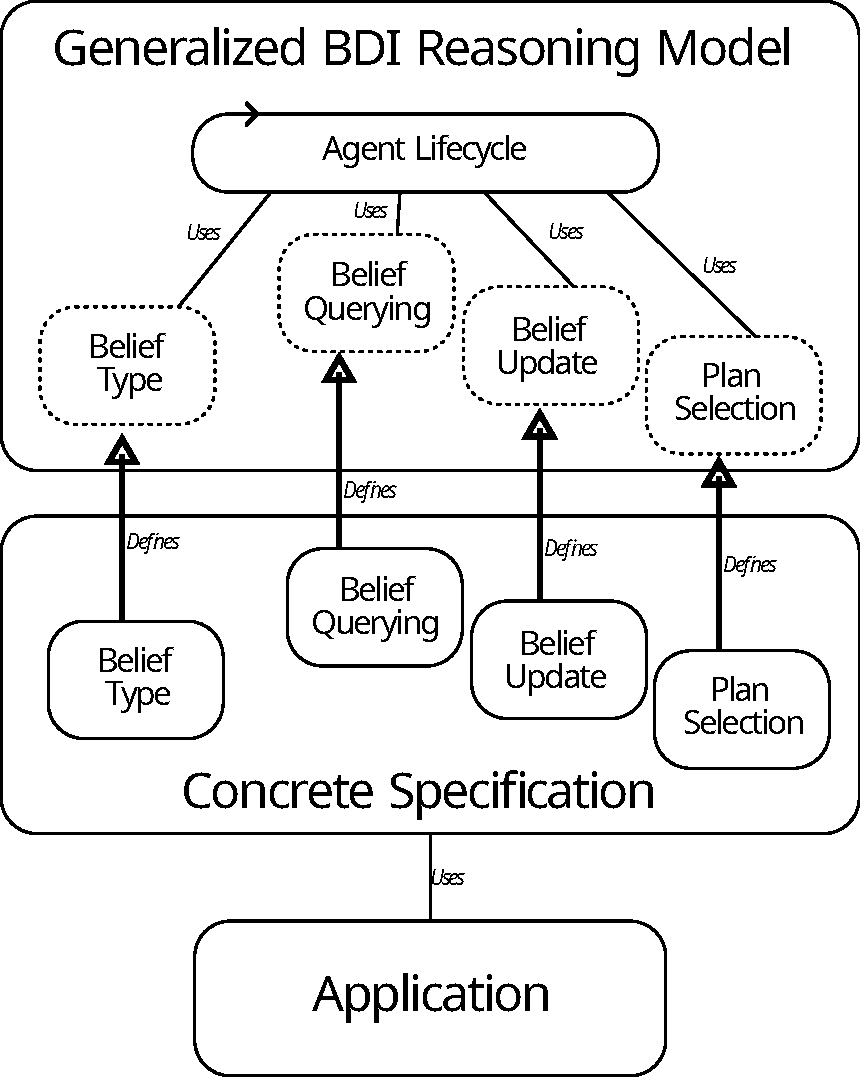
\includegraphics[width=0.5\linewidth]{figures/architecture.pdf}
  \caption{tbd}
\end{figure}

%==========================================================
\section{Discussion}
\label{sec:discussion}
%==========================================================

\sbnote{Challenges and opportunities of the approach, e.g. ontological reasoning and inference, Belief consistency, "goal" definition and management, }

%==========================================================
\section{Conclusion}
\label{sec:conclusion}
%==========================================================


%%
%% The acknowledgments section is defined using the "acknowledgments" environment
%% (and NOT an unnumbered section). This ensures the proper
%% identification of the section in the article metadata, and the
%% consistent spelling of the heading.
\begin{acknowledgments}
  \sbnote{Add Acks} 
\end{acknowledgments}

%% The declaration on generative AI comes in effect
%% in Janary 2025. See also
%% https://ceur-ws.org/GenAI/Policy.html
\section*{Declaration on Generative AI}

%   {\em Either:}\newline
%   The author(s) have not employed any Generative AI tools.
%   \newline
  
%  \noindent{\em Or (by using the activity taxonomy in ceur-ws.org/genai-tax.html):\newline}
%  During the preparation of this work, the author(s) used X-GPT-4 and Gramby in order to: Grammar and spelling check. Further, the author(s) used X-AI-IMG for figures 3 and 4 in order to: Generate images. After using these tool(s)/service(s), the author(s) reviewed and edited the content as needed and take(s) full responsibility for the publication’s content. 
\sbnote{TODO check commented text above, sicuramente usato copilot per la scrittura}

%%
%% Define the bibliography file to be used
\bibliography{bibliography}

%%
%% If your work has an appendix, this is the place to put it.
% \appendix

% \section{Online Resources}
% The sources for the ceur-art style are available via
% \begin{itemize}
% \item \href{https://github.com/yamadharma/ceurart}{GitHub},
% % \item \href{https://www.overleaf.com/project/5e76702c4acae70001d3bc87}{Overleaf},
% \item
%   \href{https://www.overleaf.com/latex/templates/template-for-submissions-to-ceur-workshop-proceedings-ceur-ws-dot-org/pkfscdkgkhcq}{Overleaf
%     template}.
% \end{itemize}

\end{document}

%%
%% End of file
